\documentclass{standalone}

\usepackage{tikz}
\usetikzlibrary{decorations.pathreplacing,calligraphy}
\usepackage{xcolor}
\colorlet{darkRed}{red!40!black}
\colorlet{darkBlue}{cyan!50!black}
\colorlet{darkYellow}{yellow!50!black}


\begin{document}

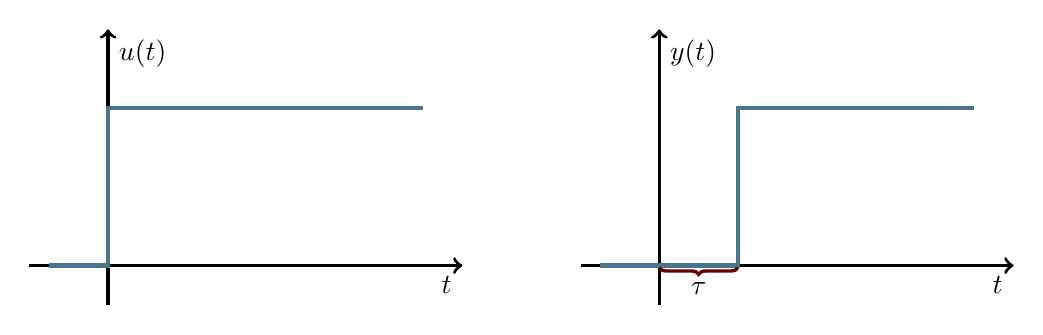
\begin{tikzpicture}[very thick]
  \draw[-to] (-1,0) -- (4.5,0) node[below left] {$t$};
  \draw[-to] (0,-0.5) -- ++(0,3.5) node[below right] {$u(t)$};
  \draw[darkBlue, ultra thick] (-.75,0) -- (0,0) -- (0,2) -- (4,2);

  \begin{scope}[xshift=7cm]
    \draw[-to] (-1,0) -- (4.5,0) node[below left] {$t$};
    \draw[-to] (0,-0.5) -- ++(0,3.5) node[below right] {$y(t)$};

    \draw[darkBlue, ultra thick] (-.75,0) -- (1,0) -- (1,2) -- (4,2);

    \draw[
      decorate,
      decoration={brace},
       draw =darkRed
    ] (1,-.025) -- (0,-.025) node[midway, below=.5mm] {$\tau$};
  \end{scope}
\end{tikzpicture}
\end{document}
